\documentclass[11pt]{article}

\usepackage{amssymb,amsmath}
\usepackage{times,psfrag,epsf,epsfig,graphics,graphicx}
\usepackage{algorithm}
\usepackage{algorithmic}

\begin{document}
\date{}

\title{PHSX 343: Assignment 1}

\author{William Jardee}

\maketitle


\section*{Problem 1}

\begin{figure}[h]
    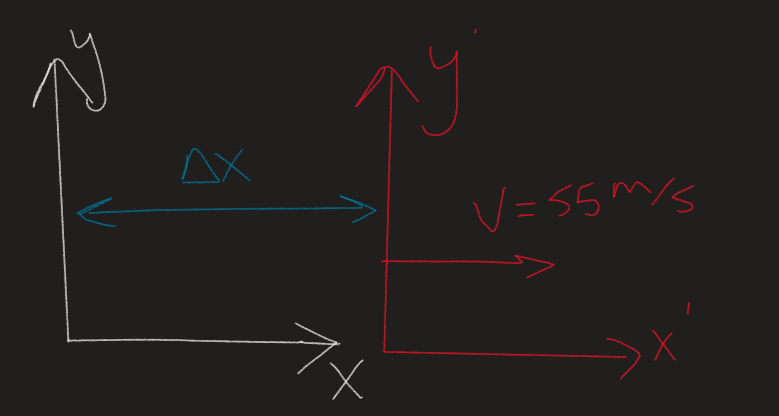
\includegraphics[width = 200]{Template/Homework1/picture 1.png}
    \label{fig:my_label}
\end{figure}\\
\noindent 
$\Delta x = (55m/s)(15s) = (825 m)$\\
$S = 1km$\\
$S' = 1km - 0.825km = 0.175km$. \\
We are in the non-relativistic realm, so the time doesn't fluctuate. So for both frames $t = 15s$.

\section*{Problem 2}

\begin{figure}[h]
    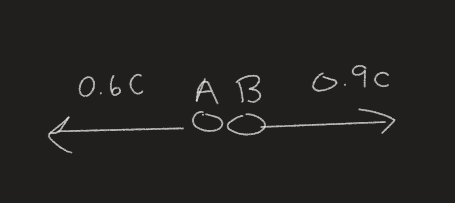
\includegraphics[width = 200]{Template/Homework1/picture 2.png}
    \label{fig:my_label}
\end{figure}\\
\noindent
$V_A = -0.6c$ and $V_B = 0.9c$\\
In the reference frame of B: $V'_A = V_A - V_B = -1.5c$\\
In the reference frame of A: $V'_B = V_B - V_A = 1.5c$\\
${V'_B} = -{V'_A} = 1.5c$\\
The speed of the two particles are the same, but the direction are opposite.

\section*{Problem 3}

\subsection*{Problem 1(a)}
$P_{tot,i} = (0.750kg)(10m/s) + 0$ and $P_{tot,f} = 0 + (0.750kg)(10m/s)$\\
$P_{tot,i} = P_{tot,f}$, so total momentum is conserved in the boat's frame.

\subsection*{Problem 1(b)}
If we name the puck initially moving as A and the other puck B:\\
Before the collision: $V_A = 7 m/s$ and $V_B = 17m/s$\\
After the collision: $V_A = 17 m/s$ and $V_B = 7m/s$\\\\
$P_{tot,i} = (0.750kg)(17m/s) + (0.750kg)(7m/s)$ and $P_{tot,f} = (0.750kg)(7m/s) + (0.750kg)(17m/s)$\\
$P_{tot,i} = P_{tot,f}$, so total momentum is conserved in the boat's frame.

\end{document}
